\documentclass[11pt, oneside]{article}   	% use "amsart" instead of "article" for AMSLaTeX format
\usepackage{geometry}                		% See geometry.pdf to learn the layout options. There are lots.
\geometry{letterpaper}                   		% ... or a4paper or a5paper or ... 
%\geometry{landscape}                		% Activate for for rotated page geometry
%\usepackage[parfill]{parskip}    		% Activate to begin paragraphs with an empty line rather than an indent
\usepackage{graphicx}				% Use pdf, png, jpg, or eps� with pdflatex; use eps in DVI mode
								% TeX will automatically convert eps --> pdf in pdflatex		
\usepackage{amssymb}
\usepackage{amsmath}
\usepackage{parskip}
\usepackage{color}

\title{Introduction to surface integrals}
%\author{The Author}
%\section{}
% \subsection*{R code}
\date{}							% Activate to display a given date or no date

\graphicspath{{/Users/telliott_admin/Dropbox/Tex/png/}}

% \begin{center} 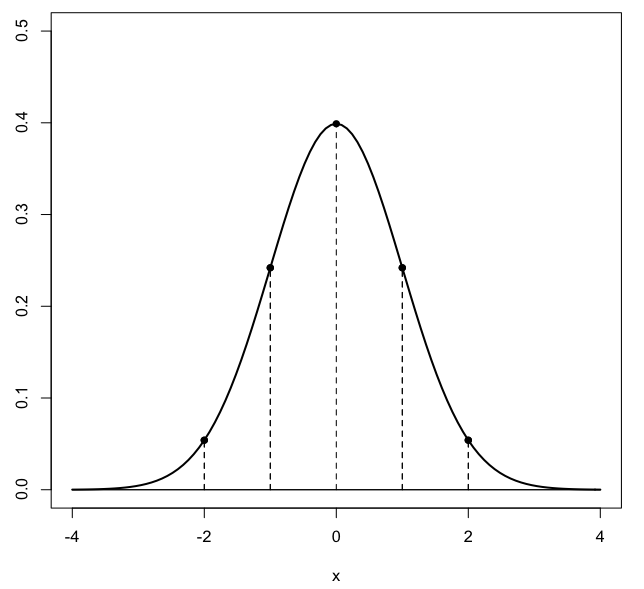
\includegraphics [scale=0.4] {gauss3.png} \end{center}
% \begin{bmatrix} a  &  b \\ c  &  d \end{bmatrix}
% \bigg |_

\begin{document}
\maketitle
\large
%\noindent
The theorem for surface integrals is that the area element is given by
\[ dS = \sqrt{(f_x)^2 + (f_y)^2 + 1} \ \ dx \ dy \]
\[ A(S) = \iint_{D} 1 \ dS =  \iint_{R} \sqrt{(f_x)^2 + (f_y)^2 + 1} \ \ dA \]
If you want to see where this comes from, you should look at the write-up for Schey Ch 2-1.  But basically what is happening is that the exchange rate between area on the surface and area in the plane is
\[ dR = \hat{\mathbf{n}} \cdot \hat{\mathbf{k}} \ dS \]
where 
\[  \hat{\mathbf{n}} = \frac{1}{\sqrt{f_x^2  + f_y^2 + 1}} \ < \ -f_x, - f_y , 1  \ > \]
\[  \hat{\mathbf{n}} \cdot \hat{\mathbf{k}} = \frac{1}{\sqrt{f_x^2  + f_y^2 + 1}} \ (1)   \]
$dS$ is larger than dA by a factor of the part of the unit normal vector that points up, this is $\cos \theta$, where $\theta$ is the angle between $\hat{\mathbf{n}}$ and $\hat{\mathbf{k}}$.
\subsection*{Plane}
A plane is almost too easy.  Suppose we take the plane which goes through the points $(2,0,0)$, $(0,2,0)$ and $(0,0,2)$ (forming an equilateral triangle with side lengths $2 \sqrt{2}$, altitude $\sqrt{3} \sqrt{2}$ and area $2 \sqrt{3}$.

The equation of the surface is $x + y + z = 2$ or $z = f(x,y) = 2 - x - y$.
The multiplicative constant is
\[ \sqrt{f_x^2  + f_y^2 + 1} = \sqrt{3} \]
The region $R$ in the plane has bounds $y=0 \rightarrow 1$ and $x=0 \rightarrow 2-y$ so we have
\[ A = \int_0^2 \int_0^{2-y} \sqrt{3} \ dx \ dy \]
\[ = \sqrt{3} \int_0^2 2 - y \ dy \]
\[ = \sqrt{3} \ (2y - \frac{1}{2}y^2) \bigg |_0^2 = 2 \sqrt{3} \]
Of course, we could put a density function or some other scalar function $G(x,y,z)$ under the integral as well.  For example $xy + z$
\[ A = \int_0^2 \int_0^{2-y} \sqrt{3} \ ( xy + z) \ dx \ dy \]
\[ A = \sqrt{3} \int_0^2 \int_0^{2-y} xy + 2 - x - y \ dx \ dy \]
\[ A = \sqrt{3} \int_0^2 ( \frac{1}{2}x^2y + 2x - \frac{1}{2}x^2 - yx) \bigg |_0^{2-y}  \ dy \]
$(2-y)^2 = 4 - 2y + y^2$, so the inner integral is
\[ \frac{1}{2}(4-2y+y^2)y + 2(2-y) - \frac{1}{2}(4-2y+y^2) - y(2-y) \]
\[ = 2y - y^2 + \frac{1}{2}y^3 + 4 - 2y - 2 + y - \frac{1}{2}y^2 - 2y + y^2 \]
\[ = \frac{1}{2}y^3 - \frac{1}{2}y^2 - y + 2 \]
Integrate and evaluate
\[ (\frac{1}{8}y^4 - \frac{1}{6}y^3 - \frac{1}{2}y^2 + 2y) \bigg |_0^2 = 2 - \frac{4}{3} - 2 + 4 =  \frac{11}{3}  \]
Remember the $\sqrt{3}$ for the final answer.

\subsection*{Paraboloid}
Our purpose here is to develop two simple examples, the surface areas of the paraboloid and the hemisphere.  For the paraboloid, consider one which has its vertex at $z=1$ and opens down
\[ z = 1 - x^2 - y^2 \]
When $z=0$ this is just $x^2 + y^2 = 1$.  We find that 
\[ f_x = -2x \]
\[ f_y = -2y \]
\[ \sqrt{f_x^2  + f_y^2 + 1} = \sqrt{4x^2 + 4y^2 + 1} \]
This would be a good time to switch to polar coordinates.
\[ x^2 + y^2 = r^2 \]
\[ \sqrt{(f_x)^2 + (f_y)^2 + 1} = \sqrt{4r^2 + 1} \]
 So we have the integral
\[ \int \int \sqrt{4r^2 + 1} \ \ r \ dr \ d \theta \]
with the $r$ term coming from the usual source. 
The inner integral is
\[ \frac{1}{12} \  (4r^2 + 1)^{3/2} \]
For the unit circle ($r=0 \rightarrow 1$), and multiplying by $2\pi$ for the outer integral, this is
\[ 2 \pi \ \frac{1}{12} \ [ \  (5)^{3/2} - 1^{3/2} ] = \frac{\pi}{6} \ [ \ 5 \sqrt{5} - 1 \ ] \]
In general, if the limits for the radius are $r=a \rightarrow r=b$ we will have
\[ \frac{\pi}{6}\ [ \ (4b^2 + 1)^{3/2} - (4a^2 + 1)^{3/2} \ ] \]

We can check this using the surface of a solid of revolution.  Turn the function to have more familiar variables.  It is $y=\sqrt{x}$.  Rotated around the $x$-axis, this solid has a cross-section at each point with circumference $2 \pi y = 2 \pi \sqrt{x}$.  The surface area is
\[ \int 2 \pi \sqrt{x} \ ds \]
The surface area element is 
\[ ds = \sqrt{1 + f'(x)^2} \ dx \]
(Looks familiar!)  So $f'(x)^2 = \frac{1}{4x}$ and we have
\[ \int 2 \pi \sqrt{x} \ \sqrt{1 + \frac{1}{4} x} \ dx \]
\[ 2 \pi \int \sqrt{x + \frac{1}{4}} \ dx \]
\[ \frac{4}{3} \pi \ (x + \frac{1}{4})^{3/2} \]
\[ \frac{\pi }{6} \ (4x + 1)^{3/2} \]
evaluated between $x=0 \rightarrow 1$, we obtain
\[ \frac{\pi }{6} \ [ \ (5)^{3/2} - 1^{3/2} \ ] \ = \frac{\pi}{6} \ [ \ 5 \sqrt{5} - 1 \ ] \]
which matches what we had by the new method.

\vspace{10 mm}

\subsection*{Hemisphere}
For the unit hemisphere we have that
\[ x^2 + y^2 + z^2 = 1 \]
\[ z = \sqrt{1 - x^2 - y^2} \]
\[ f_x = \frac{1}{z}\frac{1}{2}( -2x) = -\frac{x}{z} \]
\[ f_y = \frac{1}{z}\frac{1}{2} (-2y) = -\frac{y}{z} \]
\[ \sqrt{f_x^2  + f_y^2 + 1} = \sqrt{1 + (\frac{x}{z})^2 +  (\frac{y}{z})^2} \]
Here, the trick is to multiply on the bottom by $1/z$ and on top by $\sqrt{z^2}$
\[ = \frac{1}{z} \sqrt{z^2 + x^2 +  y^2} = \frac{1}{z}\]
So our integral is
\[ \iint_{R} \frac{1}{z} \ \ dA \]
\[ = \iint_{R} \frac{1}{\sqrt{1 - x^2 - y^2}} \ \ dA \]
This would be a good time to switch to polar coordinates.
\[ = \iint_{R} \frac{1}{\sqrt{1 - r^2}} \ r \ dr \ d \theta \]
The inner integral is 
\[ - \sqrt{1 - r^2} \]
If the limits for the radius are $r=0 \rightarrow r=1$ this is just $1$, multiplied by $2\pi$ from the outer integral.  If the sphere's radius is $\rho=a$, then there are two differences.  First, we multiply by $a/z$ above and our integral is
\[ \iint_{R} \frac{a}{z} \ \ dA \]
and then second, the inner integral is evaluated as
\[ - \sqrt{a^2 - r^2} \]
between $r=0 \rightarrow r=a$, which is  of course $a$, multiplied by by $2 a \pi$ it becomes $2 \pi a^2$ for the surface area of one-half of a sphere.

Note:  my difficulty with these problems has come from wanting to switch to cylindrical or spherical coordinates.  But this is a double integral over the region $R$ in the plane, and the appropriate choice is to switch to polar coordinates in $r$ and $\theta$.

A modification of this simple type of problem is to suppose we want the area of the object above a plane slicing through at $z=const$.  Suppose the radius of the sphere is $\rho = a$.  Then, at the simplification step above, we get
\[ = \frac{1}{z} \sqrt{z^2 + x^2 +  y^2} = \frac{a}{z}  \]
\[ a \iint_{R} \frac{1}{z} \ \ dA \]
\[ = a \iint_{R} \frac{1}{\sqrt{a^2 - x^2 - y^2}} \ \ dA \]
This would be a good time to switch to polar coordinates.
\[ = a \iint_{R} \frac{1}{\sqrt{a^2 - r^2}} \ r \ dr \ d \theta \]

What are the limits on $r$? We have
\[ z^2 = a^2 - x^2 - y^2 \]
\[ z = 1 \]
\[ x^2 + y^2 = r^2 = a^2 - 1 \]
so $r=0 \rightarrow r=\sqrt{a^2-1}$.  The inner integral is then
\[ - \sqrt{a^2 - r^2} \ \bigg |_0^{\sqrt{a^2-1}} \]
\[ = a - 1 \]
times $2 \pi a$
\[ A(S) = 2 \pi a (a-1) \]

\end{document}  